\documentclass[11pt,compress,t,notes=noshow, xcolor=table]{beamer}
\usepackage[]{graphicx}\usepackage[]{color}
% maxwidth is the original width if it is less than linewidth
% otherwise use linewidth (to make sure the graphics do not exceed the margin)
\makeatletter
\def\maxwidth{ %
  \ifdim\Gin@nat@width>\linewidth
    \linewidth
  \else
    \Gin@nat@width
  \fi
}
\makeatother

\definecolor{fgcolor}{rgb}{0.345, 0.345, 0.345}
\newcommand{\hlnum}[1]{\textcolor[rgb]{0.686,0.059,0.569}{#1}}%
\newcommand{\hlstr}[1]{\textcolor[rgb]{0.192,0.494,0.8}{#1}}%
\newcommand{\hlcom}[1]{\textcolor[rgb]{0.678,0.584,0.686}{\textit{#1}}}%
\newcommand{\hlopt}[1]{\textcolor[rgb]{0,0,0}{#1}}%
\newcommand{\hlstd}[1]{\textcolor[rgb]{0.345,0.345,0.345}{#1}}%
\newcommand{\hlkwa}[1]{\textcolor[rgb]{0.161,0.373,0.58}{\textbf{#1}}}%
\newcommand{\hlkwb}[1]{\textcolor[rgb]{0.69,0.353,0.396}{#1}}%
\newcommand{\hlkwc}[1]{\textcolor[rgb]{0.333,0.667,0.333}{#1}}%
\newcommand{\hlkwd}[1]{\textcolor[rgb]{0.737,0.353,0.396}{\textbf{#1}}}%
\let\hlipl\hlkwb

\usepackage{framed}
\makeatletter
\newenvironment{kframe}{%
 \def\at@end@of@kframe{}%
 \ifinner\ifhmode%
  \def\at@end@of@kframe{\end{minipage}}%
  \begin{minipage}{\columnwidth}%
 \fi\fi%
 \def\FrameCommand##1{\hskip\@totalleftmargin \hskip-\fboxsep
 \colorbox{shadecolor}{##1}\hskip-\fboxsep
     % There is no \\@totalrightmargin, so:
     \hskip-\linewidth \hskip-\@totalleftmargin \hskip\columnwidth}%
 \MakeFramed {\advance\hsize-\width
   \@totalleftmargin\z@ \linewidth\hsize
   \@setminipage}}%
 {\par\unskip\endMakeFramed%
 \at@end@of@kframe}
\makeatother

\definecolor{shadecolor}{rgb}{.97, .97, .97}
\definecolor{messagecolor}{rgb}{0, 0, 0}
\definecolor{warningcolor}{rgb}{1, 0, 1}
\definecolor{errorcolor}{rgb}{1, 0, 0}
\newenvironment{knitrout}{}{} % an empty environment to be redefined in TeX

\usepackage{alltt}
\newcommand{\SweaveOpts}[1]{}  % do not interfere with LaTeX
\newcommand{\SweaveInput}[1]{} % because they are not real TeX commands
\newcommand{\Sexpr}[1]{}       % will only be parsed by R



\usepackage[english]{babel}
\usepackage[utf8]{inputenc}

\usepackage{dsfont}
\usepackage{verbatim}
\usepackage{amsmath}
\usepackage{amsfonts}
\usepackage{bm}
\usepackage{csquotes}
\usepackage{multirow}
\usepackage{longtable}
\usepackage{booktabs}
\usepackage{enumerate}
\usepackage[absolute,overlay]{textpos}
\usepackage{psfrag}
\usepackage{algorithm}
\usepackage{algpseudocode}
\usepackage{eqnarray}
\usepackage{arydshln}
\usepackage{tabularx}
\usepackage{placeins}
\usepackage{tikz}
\usepackage{setspace}
\usepackage{colortbl}
\usepackage{mathtools}
\usepackage{wrapfig}
\usepackage{bm}
\usetikzlibrary{shapes,arrows,automata,positioning,calc,chains,trees, shadows}
\tikzset{
  %Define standard arrow tip
  >=stealth',
  %Define style for boxes
  punkt/.style={
    rectangle,
    rounded corners,
    draw=black, very thick,
    text width=6.5em,
    minimum height=2em,
    text centered},
  % Define arrow style
  pil/.style={
    ->,
    thick,
    shorten <=2pt,
    shorten >=2pt,}
}
\usepackage{subfig}


% Defines macros and environments
\usepackage{bbm}
% basic latex stuff
\newcommand{\pkg}[1]{{\fontseries{b}\selectfont #1}} %fontstyle for R packages
\newcommand{\lz}{\vspace{0.5cm}} %vertical space
\newcommand{\dlz}{\vspace{1cm}} %double vertical space
\newcommand{\oneliner}[1] % Oneliner for important statements
{\begin{block}{}\begin{center}\begin{Large}#1\end{Large}\end{center}\end{block}}


%new environments
\newenvironment{vbframe}  %frame with breaks and verbatim
{
 \begin{frame}[containsverbatim,allowframebreaks]
}
{
\end{frame}
}

\newenvironment{vframe}  %frame with verbatim without breaks (to avoid numbering one slided frames)
{
 \begin{frame}[containsverbatim]
}
{
\end{frame}
}

\newenvironment{blocki}[1]   % itemize block
{
 \begin{block}{#1}\begin{itemize}
}
{
\end{itemize}\end{block}
}

\newenvironment{fragileframe}[2]{  %fragile frame with framebreaks
\begin{frame}[allowframebreaks, fragile, environment = fragileframe]
\frametitle{#1}
#2}
{\end{frame}}


\newcommand{\myframe}[2]{  %short for frame with framebreaks
\begin{frame}[allowframebreaks]
\frametitle{#1}
#2
\end{frame}}

\newcommand{\remark}[1]{
  \textbf{Remark:} #1
}

\newcommand{\citebutton}[2]{%
\NoCaseChange{\resizebox{!}{9pt}{\protect\beamergotobutton{\href{#2}{#1}}}}%
}



\newenvironment{deleteframe}
{
\begingroup
\usebackgroundtemplate{\includegraphics[width=\paperwidth,height=\paperheight]{../style/color/red.png}}
 \begin{frame}
}
{
\end{frame}
\endgroup
}
\newenvironment{simplifyframe}
{
\begingroup
\usebackgroundtemplate{\includegraphics[width=\paperwidth,height=\paperheight]{../style/color/yellow.png}}
 \begin{frame}
}
{
\end{frame}
\endgroup
}\newenvironment{draftframe}
{
\begingroup
\usebackgroundtemplate{\includegraphics[width=\paperwidth,height=\paperheight]{../style/color/green.jpg}}
 \begin{frame}
}
{
\end{frame}
\endgroup
}
% https://tex.stackexchange.com/a/261480: textcolor that works in mathmode
\makeatletter
\renewcommand*{\@textcolor}[3]{%
  \protect\leavevmode
  \begingroup
    \color#1{#2}#3%
  \endgroup
}
\makeatother

% \usepackage{bbm}
% basic latex stuff
\newcommand{\pkg}[1]{{\fontseries{b}\selectfont #1}} %fontstyle for R packages
\newcommand{\lz}{\vspace{0.5cm}} %vertical space
\newcommand{\dlz}{\vspace{1cm}} %double vertical space
\newcommand{\oneliner}[1] % Oneliner for important statements
{\begin{block}{}\begin{center}\begin{Large}#1\end{Large}\end{center}\end{block}}


%new environments
\newenvironment{vbframe}  %frame with breaks and verbatim
{
 \begin{frame}[containsverbatim,allowframebreaks]
}
{
\end{frame}
}

\newenvironment{vframe}  %frame with verbatim without breaks (to avoid numbering one slided frames)
{
 \begin{frame}[containsverbatim]
}
{
\end{frame}
}

\newenvironment{blocki}[1]   % itemize block
{
 \begin{block}{#1}\begin{itemize}
}
{
\end{itemize}\end{block}
}

\newenvironment{fragileframe}[2]{  %fragile frame with framebreaks
\begin{frame}[allowframebreaks, fragile, environment = fragileframe]
\frametitle{#1}
#2}
{\end{frame}}


\newcommand{\myframe}[2]{  %short for frame with framebreaks
\begin{frame}[allowframebreaks]
\frametitle{#1}
#2
\end{frame}}

\newcommand{\remark}[1]{
  \textbf{Remark:} #1
}

\newcommand{\citebutton}[2]{%
\NoCaseChange{\resizebox{!}{9pt}{\protect\beamergotobutton{\href{#2}{#1}}}}%
}



\newenvironment{deleteframe}
{
\begingroup
\usebackgroundtemplate{\includegraphics[width=\paperwidth,height=\paperheight]{../style/color/red.png}}
 \begin{frame}
}
{
\end{frame}
\endgroup
}
\newenvironment{simplifyframe}
{
\begingroup
\usebackgroundtemplate{\includegraphics[width=\paperwidth,height=\paperheight]{../style/color/yellow.png}}
 \begin{frame}
}
{
\end{frame}
\endgroup
}\newenvironment{draftframe}
{
\begingroup
\usebackgroundtemplate{\includegraphics[width=\paperwidth,height=\paperheight]{../style/color/green.jpg}}
 \begin{frame}
}
{
\end{frame}
\endgroup
}
% https://tex.stackexchange.com/a/261480: textcolor that works in mathmode
\makeatletter
\renewcommand*{\@textcolor}[3]{%
  \protect\leavevmode
  \begingroup
    \color#1{#2}#3%
  \endgroup
}
\makeatother


%\usetheme{lmu-lecture}
\newcommand{\titlefigure}{figure/cart_tuning_nestintro_1}
\newcommand{\learninggoals}{
\item Understand the problem of overtuning
\item Be able to explain the untouched test set principle and how it motivates the idea of nested resampling}
\usepackage{../../style/lmu-lecture}

\let\code=\texttt
\let\proglang=\textsf

\setkeys{Gin}{width=0.9\textwidth}

\title{Introduction to Machine Learning}
% \author{Bernd Bischl, Christoph Molnar, Daniel Schalk, Fabian Scheipl}
\institute{\href{https://compstat-lmu.github.io/lecture_i2ml/}{compstat-lmu.github.io/lecture\_i2ml}}
\date{}

\setbeamertemplate{frametitle}{\expandafter\uppercase\expandafter\insertframetitle}



\begin{document}


% Load all R packages and set up knitr

% This file loads R packages, configures knitr options and sets preamble.Rnw as parent file
% IF YOU MODIFY THIS, PLZ ALSO MODIFY setup.Rmd ACCORDINGLY...








%! includes: tuning-tuningproblem, evaluation-resampling

\lecturechapter{Nested Resampling Motivation}
\lecture{Introduction to Machine Learning}

\begin{vbframe}{Motivation}
Selecting the best model from a set of potential candidates (e.g., different classes of learners, different hyperparameter settings, different feature sets, different preprocessing, ....) is an important part of most  machine learning problems.
\vspace{-1ex}
\begin{blocki}{Problem}
    \item We cannot evaluate our finally selected learner on the same resampling splits that we have used to perform model selection for it, e.g., to tune its hyperparameters.
    \item By repeatedly evaluating the learner on the same test set, or the same CV splits, information
      about the test set \enquote{leaks} into our evaluation.
    \item Danger of overfitting to the resampling splits / overtuning!
    \item The final performance estimate will be optimistically biased.
    \item One could also see this as a problem similar to multiple testing.
\end{blocki}
\end{vbframe}

\begin{vbframe}{Instructive and problematic example}
\begin{itemize}
    \item Assume a binary classification problem with equal class sizes.
    \item Assume a learner with hyperparameter $\lambda$.
    \item Here, the learner is a (nonsense) feature-independent classifier,
          where $\lambda$ has no effect. The learner simply
          predicts random labels with equal probability.
    \item Of course, its true generalization error is 50\%.
    \item A cross-validation of the learner (with any fixed $\lambda$) will easily show this
      (given that the partitioned data set for CV is not too small).
    \item Now let's \enquote{tune} it, by trying out 100 different $\lambda$ values.
    \item We repeat this experiment 50 times and average results.
\end{itemize}

\framebreak

\begin{knitrout}\scriptsize
\definecolor{shadecolor}{rgb}{0.969, 0.969, 0.969}\color{fgcolor}

{\centering 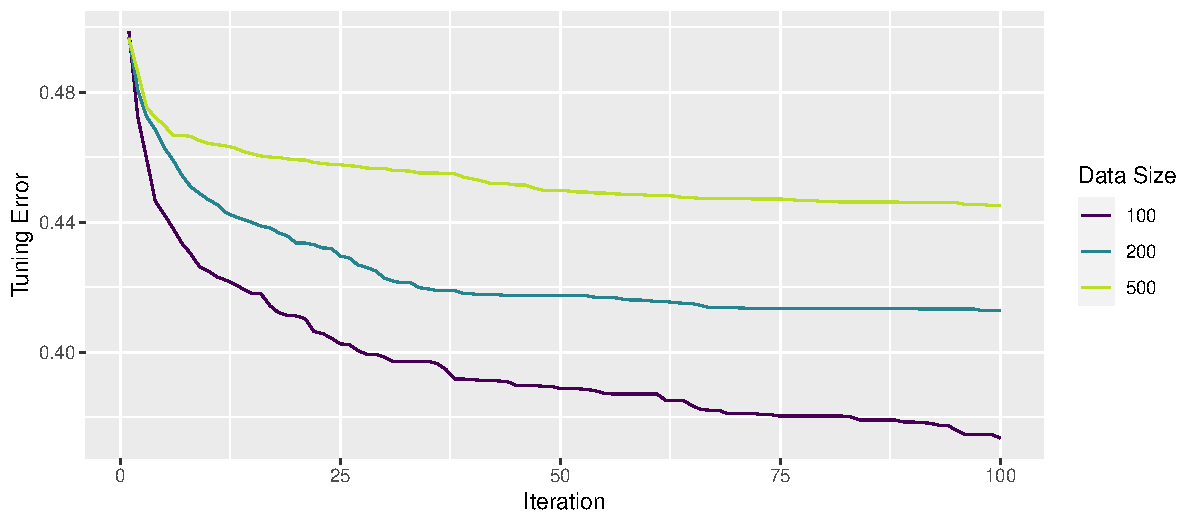
\includegraphics[width=0.95\textwidth]{figure/cart_tuning_nestintro_1} 
}
%FIGURE SOURCE: fig-cart_tuning_nestintro_1.R


\end{knitrout}

\begin{itemize}
\item Plotted is the best \enquote{tuning error} (i.e. the performance of the model with fixed $\lambda$ as evaluated by the cross-validation) after $k$ tuning iterations.
\item We have performed the experiment for different sizes of learning data
      that were cross-validated.
\end{itemize}

\begin{knitrout}\scriptsize
\definecolor{shadecolor}{rgb}{0.969, 0.969, 0.969}\color{fgcolor}

{\centering 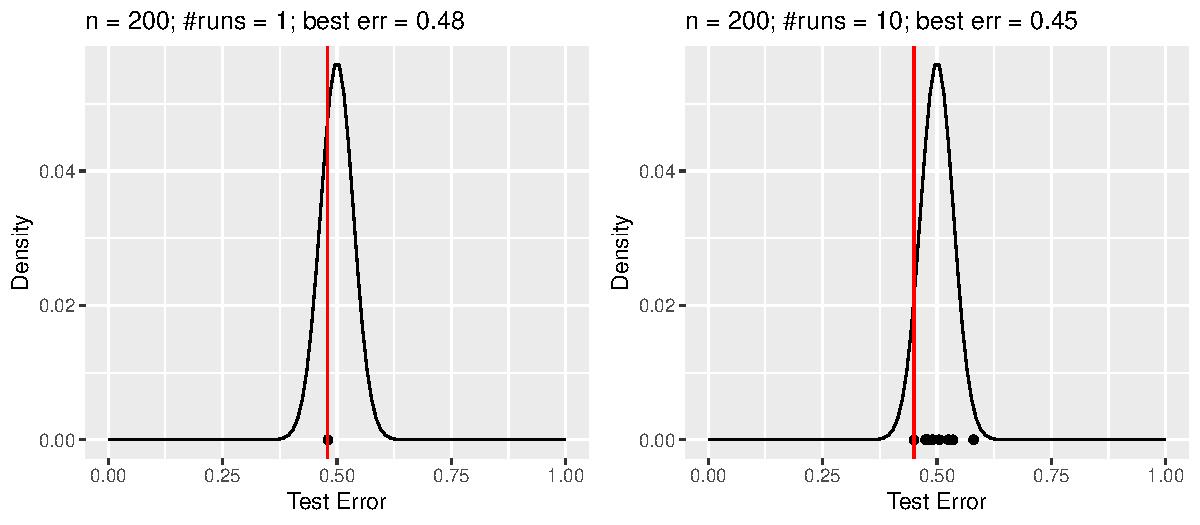
\includegraphics[width=0.95\textwidth]{figure/cart_tuning_nestintro_2} 

}
%FIGURE SOURCE: fig-cart_tuning_nestintro_2.R


\end{knitrout}

\begin{itemize}
\item For 1 experiment, the CV score will be nearly 0.5, as expected
\item We basically sample from a (rescaled) binomial distribution when we calculate error rates
\item And multiple experiment scores are also nicely arranged around the expected mean 0.5
\end{itemize}

\framebreak

\begin{knitrout}\scriptsize
\definecolor{shadecolor}{rgb}{0.969, 0.969, 0.969}\color{fgcolor}

{\centering \includegraphics[width=0.95\textwidth]{figure/cart_tuning_nestintro_
}
%FIGURE SOURCE: fig-cart_tuning_nestintro_2.R


\end{knitrout}

\begin{itemize}
\item But in tuning we take the minimum of those! So we don't really estimate the "average performance" anymore, we get an estimate of "best case" performance instead.
\item The more we sample, the more "biased" this value becomes. 
\end{itemize}
\end{vbframe}

\begin{vbframe}{Untouched Test Set Principle}
Countermeasure: simulate what actually happens in model application.

\begin{itemize}
\item All parts of the model building (including model selection,
  preprocessing) should be embedded in the model-finding process
  \textbf{on the training data}.
\item The test set should only be touched once, so we have no way of \enquote{cheating}. The test data set is only used once \emph{after} a model is completely trained, after deciding, for example, on specific hyperparameters. 

Only if we do this are the performance estimates we obtained from the test set  \textbf{unbiased estimates} of the true performance.

\framebreak

\item For steps that themselves require resampling (e.g., hyperparameter tuning) this results
  in \textbf{nested resampling}, i.e., resampling strategies for both
  \begin{itemize} 
  \item tuning: an inner resampling loop to find what works best based on training data 
  \item outer evaluation on data not used for tuning to get honest estimates of the expected performance on new data
  \end{itemize}
\end{itemize}
\end{vbframe}

\endlecture


\end{document}
